% Options for packages loaded elsewhere
\PassOptionsToPackage{unicode}{hyperref}
\PassOptionsToPackage{hyphens}{url}
\PassOptionsToPackage{dvipsnames,svgnames,x11names}{xcolor}
%
\documentclass[
  letterpaper,
]{article}

\usepackage{amsmath,amssymb}
\usepackage{lmodern}
\usepackage{setspace}
\usepackage{iftex}
\ifPDFTeX
  \usepackage[T1]{fontenc}
  \usepackage[utf8]{inputenc}
  \usepackage{textcomp} % provide euro and other symbols
\else % if luatex or xetex
  \usepackage{unicode-math}
  \defaultfontfeatures{Scale=MatchLowercase}
  \defaultfontfeatures[\rmfamily]{Ligatures=TeX,Scale=1}
\fi
% Use upquote if available, for straight quotes in verbatim environments
\IfFileExists{upquote.sty}{\usepackage{upquote}}{}
\IfFileExists{microtype.sty}{% use microtype if available
  \usepackage[]{microtype}
  \UseMicrotypeSet[protrusion]{basicmath} % disable protrusion for tt fonts
}{}
\makeatletter
\@ifundefined{KOMAClassName}{% if non-KOMA class
  \IfFileExists{parskip.sty}{%
    \usepackage{parskip}
  }{% else
    \setlength{\parindent}{0pt}
    \setlength{\parskip}{6pt plus 2pt minus 1pt}}
}{% if KOMA class
  \KOMAoptions{parskip=half}}
\makeatother
\usepackage{xcolor}
\usepackage[margin=1in]{geometry}
\setlength{\emergencystretch}{3em} % prevent overfull lines
\setcounter{secnumdepth}{-\maxdimen} % remove section numbering
% Make \paragraph and \subparagraph free-standing
\ifx\paragraph\undefined\else
  \let\oldparagraph\paragraph
  \renewcommand{\paragraph}[1]{\oldparagraph{#1}\mbox{}}
\fi
\ifx\subparagraph\undefined\else
  \let\oldsubparagraph\subparagraph
  \renewcommand{\subparagraph}[1]{\oldsubparagraph{#1}\mbox{}}
\fi


\providecommand{\tightlist}{%
  \setlength{\itemsep}{0pt}\setlength{\parskip}{0pt}}\usepackage{longtable,booktabs,array}
\usepackage{calc} % for calculating minipage widths
% Correct order of tables after \paragraph or \subparagraph
\usepackage{etoolbox}
\makeatletter
\patchcmd\longtable{\par}{\if@noskipsec\mbox{}\fi\par}{}{}
\makeatother
% Allow footnotes in longtable head/foot
\IfFileExists{footnotehyper.sty}{\usepackage{footnotehyper}}{\usepackage{footnote}}
\makesavenoteenv{longtable}
\usepackage{graphicx}
\makeatletter
\def\maxwidth{\ifdim\Gin@nat@width>\linewidth\linewidth\else\Gin@nat@width\fi}
\def\maxheight{\ifdim\Gin@nat@height>\textheight\textheight\else\Gin@nat@height\fi}
\makeatother
% Scale images if necessary, so that they will not overflow the page
% margins by default, and it is still possible to overwrite the defaults
% using explicit options in \includegraphics[width, height, ...]{}
\setkeys{Gin}{width=\maxwidth,height=\maxheight,keepaspectratio}
% Set default figure placement to htbp
\makeatletter
\def\fps@figure{htbp}
\makeatother
\newlength{\cslhangindent}
\setlength{\cslhangindent}{1.5em}
\newlength{\csllabelwidth}
\setlength{\csllabelwidth}{3em}
\newlength{\cslentryspacingunit} % times entry-spacing
\setlength{\cslentryspacingunit}{\parskip}
\newenvironment{CSLReferences}[2] % #1 hanging-ident, #2 entry spacing
 {% don't indent paragraphs
  \setlength{\parindent}{0pt}
  % turn on hanging indent if param 1 is 1
  \ifodd #1
  \let\oldpar\par
  \def\par{\hangindent=\cslhangindent\oldpar}
  \fi
  % set entry spacing
  \setlength{\parskip}{#2\cslentryspacingunit}
 }%
 {}
\usepackage{calc}
\newcommand{\CSLBlock}[1]{#1\hfill\break}
\newcommand{\CSLLeftMargin}[1]{\parbox[t]{\csllabelwidth}{#1}}
\newcommand{\CSLRightInline}[1]{\parbox[t]{\linewidth - \csllabelwidth}{#1}\break}
\newcommand{\CSLIndent}[1]{\hspace{\cslhangindent}#1}

\makeatletter
\makeatother
\makeatletter
\makeatother
\makeatletter
\@ifpackageloaded{caption}{}{\usepackage{caption}}
\AtBeginDocument{%
\ifdefined\contentsname
  \renewcommand*\contentsname{Table of contents}
\else
  \newcommand\contentsname{Table of contents}
\fi
\ifdefined\listfigurename
  \renewcommand*\listfigurename{List of Figures}
\else
  \newcommand\listfigurename{List of Figures}
\fi
\ifdefined\listtablename
  \renewcommand*\listtablename{List of Tables}
\else
  \newcommand\listtablename{List of Tables}
\fi
\ifdefined\figurename
  \renewcommand*\figurename{Figure}
\else
  \newcommand\figurename{Figure}
\fi
\ifdefined\tablename
  \renewcommand*\tablename{Table}
\else
  \newcommand\tablename{Table}
\fi
}
\@ifpackageloaded{float}{}{\usepackage{float}}
\floatstyle{ruled}
\@ifundefined{c@chapter}{\newfloat{codelisting}{h}{lop}}{\newfloat{codelisting}{h}{lop}[chapter]}
\floatname{codelisting}{Listing}
\newcommand*\listoflistings{\listof{codelisting}{List of Listings}}
\makeatother
\makeatletter
\@ifpackageloaded{caption}{}{\usepackage{caption}}
\@ifpackageloaded{subcaption}{}{\usepackage{subcaption}}
\makeatother
\makeatletter
\@ifpackageloaded{tcolorbox}{}{\usepackage[many]{tcolorbox}}
\makeatother
\makeatletter
\@ifundefined{shadecolor}{\definecolor{shadecolor}{rgb}{.97, .97, .97}}
\makeatother
\makeatletter
\makeatother
\ifLuaTeX
  \usepackage{selnolig}  % disable illegal ligatures
\fi
\IfFileExists{bookmark.sty}{\usepackage{bookmark}}{\usepackage{hyperref}}
\IfFileExists{xurl.sty}{\usepackage{xurl}}{} % add URL line breaks if available
\urlstyle{same} % disable monospaced font for URLs
\hypersetup{
  pdftitle={Trade Dependence and Militarized Interstate Disputes},
  colorlinks=true,
  linkcolor={blue},
  filecolor={Maroon},
  citecolor={Blue},
  urlcolor={Blue},
  pdfcreator={LaTeX via pandoc}}

\title{Trade Dependence and Militarized Interstate Disputes}
\author{}
\date{}

\begin{document}
\maketitle
\ifdefined\Shaded\renewenvironment{Shaded}{\begin{tcolorbox}[borderline west={3pt}{0pt}{shadecolor}, interior hidden, enhanced, breakable, frame hidden, sharp corners, boxrule=0pt]}{\end{tcolorbox}}\fi

\setstretch{2}
Does trade dependence reduce conflict between states? Debate remains
over the role and significance of economic interdependence in promoting
peace: different scholars have found that dependence increases,
decreases, and has no significant effect on the likelihood of conflict
between states. However, this research has generally relied on a broad
measure of bilateral trade dependence. This paper will delve deeper into
the effect of this economic relationship by exploring product-level
dependence. If trade dependence deters conflict between states by
increasing the expected cost of conflict through trade disruptions, we
should measure the true cost of this disruption. Rarely, if ever, do we
see states threaten to or impose total trade embargoes. Rather, states
impose trade bans on specific products that maximize the cost borne by
their opponent while minimizing the cost to their own economy. Using
this more disaggregated measure of trade dependence and a binary
logistic regression model, I find that this dependence does not have a
significant effect on the likelihood of militarized disputes between
states.

\newpage{}

The commercial peace theory maintains that trade fosters peace between
states because it makes conflict more costly. When a state is deciding
whether to initiate conflict against another state, they weigh the
benefits they expect to derive against the costs they expect to incur.
When the benefits outweigh the costs, conflict begins. Commercial peace
theory is a simple extension of this bargaining theory of conflict: the
inevitable trade disruptions caused by conflict increase the costs
states face, which decreases the likelihood that the benefits will
outweigh the costs and conflict will begin, \emph{ceteris paribus}.

Debate remains over the role played by, and significance of, bilateral
trade dependence in conflict mitigation. Recent scholarship on the topic
has begun exploring whether this ambiguity is the product of measurement
error (Chen 2021; Chatagnier and Kavaklı 2017). Within international
relations scholarship, measures of trade dependence have been defined at
a broad level, predominantly using a measure introduced by Oneal and
Russett (1997) that explores total trade between two states relative to
their gross domestic product (GDP) (Chen 2021; Flores-Macías and Kreps
2013; Gartzke and Westerwinter 2016; Kinne 2012; Lupu and Traag 2013;
Pevehouse 2004). However, a more disaggregated approach to trade
dependence is worth exploring. We are interested in understanding how
trade dependence can deter conflict. Rarely (if ever) do states threaten
to sever their entire trade relationship with another state. Rather, we
regularly see states threaten or enact trade bans on particular
products. In fact, states often threaten to inflict the greatest harm on
their rival whilst minimizing the costs they will face. A broad
understanding of trade dependence does not capture the real threat a
potential aggressor faces. A more accurate measure of this factor is
product-level trade dependence. Asymmetries at this level have been used
as a foreign policy mechanism to deter or punish rival states.

Before we explore this dynamic in detail, let us step out in detail the
process we seek better understand. First, tensions between two states
builds. This could be for a number of reasons, including historical
animosity, a diplomatic spat over a regional or global issue, or
domestic political interests prompting an controversial bilateral
foreign policy. The threatened state issues a formal request to the
initiating state to change or reverse their policy actions. The
initiating state refuses: the incentives for enacting the controversial
policy continue to outweigh the cost of a soured relationship with the
threatened state. The threatened state responds by threatening to adopt
punitive policies towards the initiator, including trade embargoes on
specific products on which the initiator depends. Here, the initiator's
expected costs from pursuing this policy change: they know that if they
continue along this path they will likely face economic costs in the
form of trade disruptions. Does this deter them? Many scholars would
ask: how costly is this disruption? This paper will answer this
question. If the costs are not so great, the initiator may respond to
this threat through further escalation, including through a militarized
dispute. International relations scholarship uses this broad measure of
conflict to include actions that sit below invasion or war. This is
often the precursor to full-scale interstate war. States use these
actions as an extreme signal of their intent to escalate a dispute to
war, hoping to deter their opponent.

We are interested in the relationship between trade dependence and this
pre-cursor to war. Certainly, if two states are at war with one another,
we should expect trade to nearly, if not entirely, cease between them.
However, we should not expect trade to entirely cease between states
when they are still circling each other, hoping to achieve their most
desired policy outcome and avoid war. Tying a measure of the entire
trade relationship to whether or not states initiate militarized
interstate disputes (not war) against each other misses this important
distinction. This paper seeks to address this.

\hypertarget{trade-dependence-and-militarized-conflict}{%
\subsection{Trade dependence and militarized
conflict}\label{trade-dependence-and-militarized-conflict}}

Returning to our motivating question: does trade dependence deter states
from initiating militarized conflict against each other? The commercial
peace theory argues that trade dependence increases the expected cost of
initiating conflict against a trade partner, decreasing the expected net
benefits derived from such an action and, therefore, reducing the
likelihood a state will initiate conflict. This leads to the following
testable hypothesis:

\begin{quote}
H1: As product-level trade dependence between two states increases, the
likelihood that a state will initiate militarized conflict against its
trade partner decreases.
\end{quote}

\hypertarget{research-design}{%
\subsection{Research design}\label{research-design}}

\hypertarget{scope}{%
\subsubsection{Scope}\label{scope}}

This analysis focuses on all directed state dyads in 2013 and 2014. This
includes 74,884 observations. We are interested in whether or not a
trade dependent state initiates conflict against another state. This is
a directed question. We need to know whether the potential initiator is
dependent on their opponent, not simply whether either partner has a
dependence on the other.

The narrow timeframe included in this analysis is driven by data
constraints. I only have access to complete trade and militarized
interstate dispute data for 2013 and 2014. A natural first step for
extending this analysis is including a broader timeframe in the
analysis.

\hypertarget{dependent-variable}{%
\subsubsection{Dependent variable}\label{dependent-variable}}

My dependent variable focuses on the onset of militarized interstate
disputes (MIDs), or events in which one or more states threaten,
display, or use force against another state or states. If state \(i\)
initiated the MID against state \(j\) in a given year, this variable is
coded 1. Otherwise, it receives a value of 0.

The data come from version five of Palmer et al's (2022) Militarized
Interstate Dispute data collection. This dataset includes all known MIDs
from 1816-2014, recorded at the participant level. Between 2013 and
2014, 135 MIDs were initiated.

\hypertarget{independent-variables-of-interest}{%
\subsubsection{Independent variables of
interest}\label{independent-variables-of-interest}}

My primary independent variable of interest is bilateral trade
dependence. This paper introduces a novel measure of this dependence.
Rather than looking at the balance of trade in total imports, exports,
or trade value, I measure dependence in trade of specific products. This
more fine-grained approach to measuring trade dependence allows us to
examine more precisely the potential costs an initiator expects to incur
if they escalate a dispute to a MID.

To do this, I adopt the classical structure proposed by Oneal and
Russett (1997) but adapt it to trade in each product. I use bilateral
annual export and import data provided by UN Comtrade. Commodities are
grouped according to the standard two digit harmonized system. For
example, all live animals, including horses, bovines, swine, sheep, and
goats, are grouped together into a category called \emph{animals -
live}. My theory assumes a degree of substitution within this group. It
would be interesting to explore the level of granularity required to
meaningfully make this assumption. Sadly, this is difficult to test
because we lose data completeness as we increase granularity.

Formally, my measure of trade dependence is defined as the total imports
and exports from state \(i\) to (or from) state \(j\) for a given
commodity in a given year relative to state \(i\)'s GDP for that year.

\[
r_{ij,p,t} = \frac{m_{ij,p,t} + x_{ij,p,t}}{GDP_{i,t}}
\]

Where \(j\) is the trade partner and \(p\) is the product. This value is
measured for each year, \(t\).

In 2013 and 2014, product-level trade dependence ranged from 0\% to
36\%, with an average level of trade dependence of 0.09\%. The most
dependent pairing is between Sudan and United Arab Emirates: Sudan's
trade in natural, cultured pearls; precious, semi-precious stones;
precious metals, metals clad with precious metal, and articles thereof;
imitation jewellery; coin with United Arab Emirates amounts to 36\% of
Sudan's GDP in 2014.

States trade in a large number of commodities. For each directed state
dyad, we get the same number of measures of dependence as products
traded between them. We need to reduce this to a single measure of
dependence. I use the product with the highest value of dependence
between states \(i\) and \(j\). State \(j\) will strategically select
the product or products that maximize the cost state \(i\) should expect
to incur in retaliation for escalating tensions. The trade in a product
on which state \(i\) is most dependent is a good candidate for this
strategic threat or imposition of a trade embargo.\footnote{I tested
  five options for this aggregation: the minimum, the 25th percentile,
  the average, the 75th percentile, and the maximum level of trade
  dependence between two states. Let's first discuss the logic of the
  extremes: the minimum and maximum values. The minimum value represents
  the lowest possible cost state \(j\) could threaten to impose on state
  \(i\) in a given year. If this is relatively high, state \(i\) is
  probably very trade dependent on state \(j\). This should be a very
  strong measure of dependence. However, state \(j\) is unlikely to
  threaten to stop trade in this commodity. Remember, they aim to impose
  the greatest possible cost on state \(i\) whilst minimizing the cost
  to themselves. Perhaps a better candidate is trade in the most
  dependent commodity. To qualify these measures, I also also tested
  intermediate measures of dependence: the 25th, 50th, and 75th
  percentiles of trade dependence across all traded commodities. These
  measures perhaps better capture the dynamics at play with the extreme
  measures whilst allowing state \(j\) to minimize the cost it bears and
  also to select a number of commodities to disrupt, not just one. I
  found that the maximum, 75th percentile, and average measures of trade
  dependence were statistically significant to initiation of MIDs. In
  fact, the average measure of trade dependence produced the strongest
  effect on MID initiation. However, I am not sure that these abstracted
  measures of trade dependence are in the spirit of my theory or
  question. I hope to provide a more specific measure of trade
  dependence. I select the maximum value for theoretical reasons.
  Happily, I find a statistically significant relationship that I can
  explore.}

This measure allows me to focus on trade in goods that are critical to
the potential initiator. I argue that this better represents the true
cost they expect to incur if they escalate tensions with a trade partner
to a MID.

\hypertarget{control-variables}{%
\subsubsection{Control variables}\label{control-variables}}

Following other literature exploring this question, I include several
control variables. I include a binary variable accounting for whether
the dyad includes states that share a land border. I also include two
variables providing each state's level of democracy.

\hypertarget{results}{%
\subsection{Results}\label{results}}

Let's look at the relationship between the predicted probability that
state \(i\) will initiate a MID with state \(j\) for a given level of
product-level trade dependence. First, I will compare the relationship
between MID initiation and product-level and broad, total trade
dependence. I will then include traditional controls for a state's
decision to initiate a MID against a rival to see whether trade
dependence is a significant factor in this complex decision.

First, let us compare the relationship between MID initiation and
product-level trade dependence compared to the relationship estimated
using the more traditional, broad measure of trade dependence.

\textbf{See Appendix for Table 1}

I used a binary logistic regression model to predict the probability
that state \(i\) initiates a MID against state \(j\) for a given level
of trade dependence. Using product-level trade dependence, I find that
increasing dependence by one percentage point \textbf{increases} the
odds that state \(i\) will initiate MID against state \(j\) by 1.19 on
average. This relationship is highly statistically significant. This
more fine-grained measure of trade dependence predicts a stronger
relationship between conflict and trade dependence than the more
tradition and broad-based approach. Using total trade dependence, I find
that increasing dependence by one percentage point increases the odds
that state \(i\) will initiate MID against state \(j\) by 1.09 on
average.

\emph{Figure 1} illustrates the different predicted probabilities that
state \(i\) will initiate an MID against state \(j\) for each possible
level trade dependence between no dependence (0 percent) and total
dependence (100 percent).\footnote{Any prediction made for a level of
  trade dependence above 36\% for product-level dependence and 71\% for
  total trade dependence is an out of sample prediction.}

\textbf{See Appendix for Figure 1}

It is worth noting that product-level trade dependence predicts a much
more aggressive relationship between conflict and trade dependence: the
point at which MIDs are predicted to be more likely than not is at 36\%
for product-level trade dependence and 71\% for total trade dependence.

Moving from these base models to ones that incorporate traditional
controls for MIDs and trade relationships, we learn that the
relationship between conflict and trade dependence is not significant.

\textbf{See Appendix for Table 2}

For both product-level and total trade dependence, the odds that state
\(i\) will initiate an MID against state \(j\) remain positive; however,
the statistical significance of this relationship drops well below
traditional thresholds. Significant determinants of conflict include
contiguity and state \(i\)'s level of democracy. I find that state \(i\)
is less to initiate an MID against a state with which it shares a land
border, on average holding all else constant. I also find that as state
\(i\) becomes more democratic, it is less likely to initiate a MID
against state \(j\). Interestingly, I find that state \(j\)'s level of
democracy does not appear to be a significant factor in state \(i\)'s
decision to initiate an MID.

\newpage{}

\hypertarget{appendix}{%
\subsection{Appendix}\label{appendix}}

\hypertarget{regression-results}{%
\subsubsection{Regression results}\label{regression-results}}

\begin{longtable}[]{@{}
  >{\raggedright\arraybackslash}p{(\columnwidth - 12\tabcolsep) * \real{0.3265}}
  >{\centering\arraybackslash}p{(\columnwidth - 12\tabcolsep) * \real{0.0816}}
  >{\centering\arraybackslash}p{(\columnwidth - 12\tabcolsep) * \real{0.1224}}
  >{\centering\arraybackslash}p{(\columnwidth - 12\tabcolsep) * \real{0.1327}}
  >{\centering\arraybackslash}p{(\columnwidth - 12\tabcolsep) * \real{0.0816}}
  >{\centering\arraybackslash}p{(\columnwidth - 12\tabcolsep) * \real{0.1224}}
  >{\centering\arraybackslash}p{(\columnwidth - 12\tabcolsep) * \real{0.1327}}@{}}
\caption{Base models }\tabularnewline
\toprule()
\begin{minipage}[b]{\linewidth}\raggedright
\textbf{Characteristic}
\end{minipage} & \begin{minipage}[b]{\linewidth}\centering
\textbf{OR}
\end{minipage} & \begin{minipage}[b]{\linewidth}\centering
\textbf{95\% CI}
\end{minipage} & \begin{minipage}[b]{\linewidth}\centering
\textbf{p-value}
\end{minipage} & \begin{minipage}[b]{\linewidth}\centering
\textbf{OR}
\end{minipage} & \begin{minipage}[b]{\linewidth}\centering
\textbf{95\% CI}
\end{minipage} & \begin{minipage}[b]{\linewidth}\centering
\textbf{p-value}
\end{minipage} \\
\midrule()
\endfirsthead
\toprule()
\begin{minipage}[b]{\linewidth}\raggedright
\textbf{Characteristic}
\end{minipage} & \begin{minipage}[b]{\linewidth}\centering
\textbf{OR}
\end{minipage} & \begin{minipage}[b]{\linewidth}\centering
\textbf{95\% CI}
\end{minipage} & \begin{minipage}[b]{\linewidth}\centering
\textbf{p-value}
\end{minipage} & \begin{minipage}[b]{\linewidth}\centering
\textbf{OR}
\end{minipage} & \begin{minipage}[b]{\linewidth}\centering
\textbf{95\% CI}
\end{minipage} & \begin{minipage}[b]{\linewidth}\centering
\textbf{p-value}
\end{minipage} \\
\midrule()
\endhead
(Intercept) & 0.00 & 0.00, 0.00 & \textless0.001 & 0.00 & 0.00, 0.00 &
\textless0.001 \\
Trade dependence, product-level & 1.19 & 1.13, 1.25 & \textless0.001 & &
& \\
Trade dependence, total trade & & & & 1.09 & 1.07, 1.12 &
\textless0.001 \\
\bottomrule()
\end{longtable}

\begin{longtable}[]{@{}
  >{\raggedright\arraybackslash}p{(\columnwidth - 12\tabcolsep) * \real{0.3265}}
  >{\centering\arraybackslash}p{(\columnwidth - 12\tabcolsep) * \real{0.0816}}
  >{\centering\arraybackslash}p{(\columnwidth - 12\tabcolsep) * \real{0.1224}}
  >{\centering\arraybackslash}p{(\columnwidth - 12\tabcolsep) * \real{0.1327}}
  >{\centering\arraybackslash}p{(\columnwidth - 12\tabcolsep) * \real{0.0816}}
  >{\centering\arraybackslash}p{(\columnwidth - 12\tabcolsep) * \real{0.1224}}
  >{\centering\arraybackslash}p{(\columnwidth - 12\tabcolsep) * \real{0.1327}}@{}}
\caption{Controlled models }\tabularnewline
\toprule()
\begin{minipage}[b]{\linewidth}\raggedright
\textbf{Characteristic}
\end{minipage} & \begin{minipage}[b]{\linewidth}\centering
\textbf{OR}
\end{minipage} & \begin{minipage}[b]{\linewidth}\centering
\textbf{95\% CI}
\end{minipage} & \begin{minipage}[b]{\linewidth}\centering
\textbf{p-value}
\end{minipage} & \begin{minipage}[b]{\linewidth}\centering
\textbf{OR}
\end{minipage} & \begin{minipage}[b]{\linewidth}\centering
\textbf{95\% CI}
\end{minipage} & \begin{minipage}[b]{\linewidth}\centering
\textbf{p-value}
\end{minipage} \\
\midrule()
\endfirsthead
\toprule()
\begin{minipage}[b]{\linewidth}\raggedright
\textbf{Characteristic}
\end{minipage} & \begin{minipage}[b]{\linewidth}\centering
\textbf{OR}
\end{minipage} & \begin{minipage}[b]{\linewidth}\centering
\textbf{95\% CI}
\end{minipage} & \begin{minipage}[b]{\linewidth}\centering
\textbf{p-value}
\end{minipage} & \begin{minipage}[b]{\linewidth}\centering
\textbf{OR}
\end{minipage} & \begin{minipage}[b]{\linewidth}\centering
\textbf{95\% CI}
\end{minipage} & \begin{minipage}[b]{\linewidth}\centering
\textbf{p-value}
\end{minipage} \\
\midrule()
\endhead
(Intercept) & 0.00 & 0.00, 0.00 & \textless0.001 & 0.00 & 0.00, 0.00 &
\textless0.001 \\
Trade dependence, product-level & 1.05 & 0.96, 1.12 & 0.2 & & & \\
Contiguous & 69.7 & 48.6, 101 & \textless0.001 & 71.3 & 49.5, 103 &
\textless0.001 \\
Democracy, state i & 0.13 & 0.06, 0.27 & \textless0.001 & 0.13 & 0.06,
0.27 & \textless0.001 \\
Democracy, state j & 1.02 & 0.49, 2.11 & \textgreater0.9 & 1.00 & 0.48,
2.08 & \textgreater0.9 \\
Trade dependence, total trade & & & & 1.00 & 0.97, 1.03 & 0.8 \\
\bottomrule()
\end{longtable}

\hypertarget{comparison-of-product-level-and-total-trade-dependence-results}{%
\subsubsection{Comparison of product-level and total trade dependence
results}\label{comparison-of-product-level-and-total-trade-dependence-results}}

\begin{figure}

{\centering 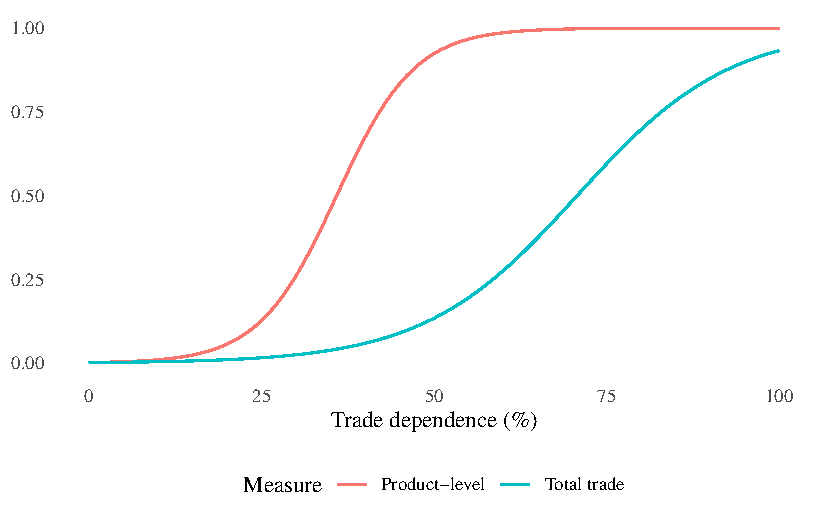
\includegraphics{article_files/figure-pdf/unnamed-chunk-4-1.pdf}

}

\caption{Predicted probability of MID given product-level trade
dependence}

\end{figure}

\newpage{}

\hypertarget{bibliography}{%
\subsection*{Bibliography}\label{bibliography}}
\addcontentsline{toc}{subsection}{Bibliography}

\hypertarget{refs}{}
\begin{CSLReferences}{1}{0}
\leavevmode\vadjust pre{\hypertarget{ref-chatagnier2017}{}}%
Chatagnier, J. Tyson, and Kerim Can Kavaklı. 2017. {``From {Economic
Competition} to {Military Combat}: {Export Similarity} and
{International Conflict}.''} \emph{The Journal of Conflict Resolution}
61 (7): 1510--36. \url{https://www.jstor.org/stable/26363938}.

\leavevmode\vadjust pre{\hypertarget{ref-chen2021}{}}%
Chen, Frederick R. 2021. {``Extended {Dependence}: {Trade}, {Alliances},
and {Peace}.''} \emph{The Journal of Politics} 83 (1): 246--59.
\url{https://doi.org/10.1086/709149}.

\leavevmode\vadjust pre{\hypertarget{ref-flores-macias2013b}{}}%
Flores-Macías, Gustavo A., and Sarah E. Kreps. 2013. {``The {Foreign
Policy Consequences} of {Trade}: {China}'s {Commercial Relations} with
{Africa} and {Latin America}, 1992--2006.''} \emph{The Journal of
Politics} 75 (2): 357--71.
\url{https://doi.org/10.1017/S0022381613000066}.

\leavevmode\vadjust pre{\hypertarget{ref-gartzke2016}{}}%
Gartzke, Erik, and Oliver Westerwinter. 2016. {``The Complex Structure
of Commercial Peace Contrasting Trade Interdependence, Asymmetry, and
Multipolarity.''} \emph{Journal of Peace Research} 53 (3): 325--43.
\url{https://www.jstor.org/stable/43920593}.

\leavevmode\vadjust pre{\hypertarget{ref-kinne2012a}{}}%
Kinne, Brandon J. 2012. {``Multilateral {Trade} and {Militarized
Conflict}: {Centrality}, {Openness}, and {Asymmetry} in the {Global
Trade Network}.''} \emph{The Journal of Politics} 74 (1): 308--22.
\url{https://doi.org/10.1017/S002238161100137X}.

\leavevmode\vadjust pre{\hypertarget{ref-lupu2013}{}}%
Lupu, Yonatan, and Vincent A. Traag. 2013. {``Trading {Communities}, the
{Networked Structure} of {International Relations}, and the {Kantian
Peace}.''} \emph{The Journal of Conflict Resolution} 57 (6): 1011--42.
\url{https://www.jstor.org/stable/24545601}.

\leavevmode\vadjust pre{\hypertarget{ref-oneal1997}{}}%
Oneal, John R., and Bruce M. Russet. 1997. {``The Classical Liberals
Were Right: Democracy, Interdependence, and Conflict, 1950-1985.''}
\emph{International Studies Quarterly} 41 (2): 267--94.
\url{https://doi.org/10.1111/1468-2478.00042}.

\leavevmode\vadjust pre{\hypertarget{ref-palmer2022}{}}%
Palmer, Glenn, Roseanne W McManus, Vito D'Orazio, Michael R Kenwick,
Mikaela Karstens, Chase Bloch, Nick Dietrich, Kayla Kahn, Kellan Ritter,
and Michael J Soules. 2022. {``The {Mid5 Dataset}, 2011--2014:
{Procedures}, Coding Rules, and Description.''} \emph{Conflict
Management and Peace Science} 39 (4): 470--82.
\url{https://doi.org/10.1177/0738894221995743}.

\leavevmode\vadjust pre{\hypertarget{ref-pevehouse2004}{}}%
Pevehouse, Jon C. 2004. {``Interdependence {Theory} and the
{Measurement} of {International Conflict}.''} \emph{The Journal of
Politics} 66 (1): 247--66.
\url{https://doi.org/10.1046/j.1468-2508.2004.00150.x}.

\end{CSLReferences}



\end{document}
